
\documentclass[11pt]{article}


\usepackage{geometry}
\geometry{a4paper,margin=3cm}

\usepackage{graphicx}

\usepackage{enumitem}
\DeclareGraphicsExtensions{.pdf,.png,.jpg}


\begin{document}




\title{Signal Green Initial Report}

\author{Waqar Aziz, James Kerr, Adeela Saalim, Andrea Senf, Yoann Strigini}

\maketitle 


\section{PROJECT DESCRIPTION}


\subsection{AIMS FOR PROJECT}

Our aim is to create a traffic simulation software where we can test various traffic management strategies that will teach us new skills and receive full marks. 
\\ \\
This means we will demonstrate our ability to use GitHub and other common engineering tools to create a vehicle simulation. It includes working together as a team and learning from each other. We will experience developing a software that is bigger than any of us could have created by ourselves in the given time. 


\subsection{STRATEGY}

\subsubsection*{SOFTWARE DEVELOPMENT PROCESS}

During the first week we analysed the specifications and identified a set of requirements, which we divided into two levels of priorities. The week of 23 February our program will at minimum run a basic simulation, and the group will assess our progress. We 
will then set final goals and specifications for our finished project, which are set to be complete the week of 2nd March. Low priority functionality may be implemented after core requirements have been released and successfully tested, and should be finished by 
9th March.
\\ \\ 
SCRUM is the methodology of choice as it provides the ability to quickly react to problems minimizing risks of failure. Furthermore, given that we all work/study full-time, SCRUM provides the transparency that is essential to know at any stage that the project is on track.


\begin{figure}[gantt8Feb]
	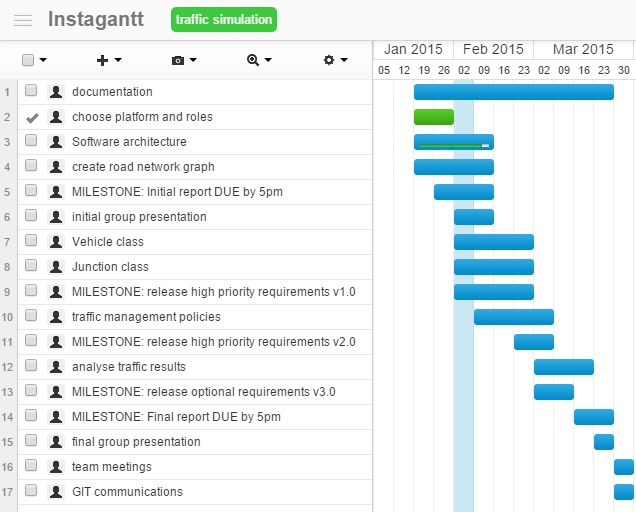
\includegraphics[scale=0.9]{gantt8Feb}
%	\centering
	\caption{Gantt chart showing expected progress}
	\centering

\end{figure}


\subsubsection*{PROGRAMMING ENVIRONMENT}

After forming the team we conducted some research in order to decide how to model the software and select tools that would provide the most effective environment.
\\ \\
We decided to use Agent-Based Modeling (ABM) rather than Object Oriented Programming (OOP) because we can model the system as a set of interacting agents (such as cars and traffic lights) which exist on an environment (the road network) and are capable behavioural adaptation, providing a realistic simulation.
\\ \\
For an ABM framework, we decided to use the RePast Simphony 2.2. It is flexible, allows module replacement if we desire, and is more recent than RePastJ. As IDE we are using the Eclipse editor because it comes set up with Simphony and it is commonly used.
\\ \\
We further considered and decided against coding an entire ABM software ourselves because would not leave sufficient time 
to complete other desired project requirements. We considered and decided against NetLogo because although it has many preexisting models, it is rather restrictive; there was also concern about the final appearance of the project.
\\ \\
Finally, we agreed on using Java because everyone on the team is experienced in using it and java is commonly used for similar applications in industry. Its ease of use compared to C++ will help us expedite programming progress.

\subsubsection*{COMMUNICATION TOOLS}

We are communicating and documenting via WhatsApp, Asana, and Instagantt, and thus far we have held weekly team meetings in person at KCL to discuss what we have researched, make decisions, and divide tasks.
\\ \\
Every week we have a SCRUM standup to ensure we all understand what progress is happening. We update Asana with comments and tasks, which automatically updates our corresponding Gantt chart in Instagantt.


\subsection{CURRENT PROGRESS}

Our team is functioning on GitHub and we are currently coding the architecture and environment. The basics of choosing and learning new enviornments is complete, and we are now focused on making progress with the program itself and continuing documentation. 
We are coding the Road Network as well as the Car and Junction classes.

%\newpage


\section{PROJECT ORGANISATION}

\subsection{TEAM WORK}

We communicate in person and via our selected communication tools.  Team members 
volunteer or recommend peers for tasks that play to that team member's strength or where 
that person would like to learn new skills.


\subsection{ROLES}

James and Yoann are focusing on the software architecture and vehicle classes. Waqar and 
Adeela are focusing on creating the road map components. Andrea is coordinator for GitHub 
purposes and is creating documentation and reporting. All team members will participate 
in testing and analysis.


\subsection{PEER ASSESSMENT}

We expect everyone to carry roughly equal amounts of work and so we plan to divide team 
points equally between us. If we have concerns that this is not happening, we will 
discuss it so there will not be surprises in our assessment of each other at the end of term.


\subsection{CONFLICTS}

Concerns or issues between team members should be discussed between the members within 
a reasonable time of noticing the problem. This is to prevent surprises when members 
evaluate each other at the end of the project, and to minimize friction between 
group members.
\\ \\
We anticipate the load should be shared fairly equally between members and 
this is considered when taking tasks during team meetings. If a member feels 
they are doing more work than others, this should be communicated to the group so action 
can be taken while there is time to remedy the issue.



\end{document}
